\documentclass[twoside]{book}

% Packages required by doxygen
\usepackage{fixltx2e}
\usepackage{calc}
\usepackage{doxygen}
\usepackage[export]{adjustbox} % also loads graphicx
\usepackage{graphicx}
\usepackage[utf8]{inputenc}
\usepackage{makeidx}
\usepackage{multicol}
\usepackage{multirow}
\PassOptionsToPackage{warn}{textcomp}
\usepackage{textcomp}
\usepackage[nointegrals]{wasysym}
\usepackage[table]{xcolor}

% Font selection
\usepackage[T1]{fontenc}
\usepackage[scaled=.90]{helvet}
\usepackage{courier}
\usepackage{amssymb}
\usepackage{sectsty}
\renewcommand{\familydefault}{\sfdefault}
\allsectionsfont{%
  \fontseries{bc}\selectfont%
  \color{darkgray}%
}
\renewcommand{\DoxyLabelFont}{%
  \fontseries{bc}\selectfont%
  \color{darkgray}%
}
\newcommand{\+}{\discretionary{\mbox{\scriptsize$\hookleftarrow$}}{}{}}

% Page & text layout
\usepackage{geometry}
\geometry{%
  a4paper,%
  top=2.5cm,%
  bottom=2.5cm,%
  left=2.5cm,%
  right=2.5cm%
}
\tolerance=750
\hfuzz=15pt
\hbadness=750
\setlength{\emergencystretch}{15pt}
\setlength{\parindent}{0cm}
\setlength{\parskip}{3ex plus 2ex minus 2ex}
\makeatletter
\renewcommand{\paragraph}{%
  \@startsection{paragraph}{4}{0ex}{-1.0ex}{1.0ex}{%
    \normalfont\normalsize\bfseries\SS@parafont%
  }%
}
\renewcommand{\subparagraph}{%
  \@startsection{subparagraph}{5}{0ex}{-1.0ex}{1.0ex}{%
    \normalfont\normalsize\bfseries\SS@subparafont%
  }%
}
\makeatother

% Headers & footers
\usepackage{fancyhdr}
\pagestyle{fancyplain}
\fancyhead[LE]{\fancyplain{}{\bfseries\thepage}}
\fancyhead[CE]{\fancyplain{}{}}
\fancyhead[RE]{\fancyplain{}{\bfseries\leftmark}}
\fancyhead[LO]{\fancyplain{}{\bfseries\rightmark}}
\fancyhead[CO]{\fancyplain{}{}}
\fancyhead[RO]{\fancyplain{}{\bfseries\thepage}}
\fancyfoot[LE]{\fancyplain{}{}}
\fancyfoot[CE]{\fancyplain{}{}}
\fancyfoot[RE]{\fancyplain{}{\bfseries\scriptsize Generated by Doxygen }}
\fancyfoot[LO]{\fancyplain{}{\bfseries\scriptsize Generated by Doxygen }}
\fancyfoot[CO]{\fancyplain{}{}}
\fancyfoot[RO]{\fancyplain{}{}}
\renewcommand{\footrulewidth}{0.4pt}
\renewcommand{\chaptermark}[1]{%
  \markboth{#1}{}%
}
\renewcommand{\sectionmark}[1]{%
  \markright{\thesection\ #1}%
}

% Indices & bibliography
\usepackage{natbib}
\usepackage[titles]{tocloft}
\setcounter{tocdepth}{3}
\setcounter{secnumdepth}{5}
\makeindex

% Hyperlinks (required, but should be loaded last)
\usepackage{ifpdf}
\ifpdf
  \usepackage[pdftex,pagebackref=true]{hyperref}
\else
  \usepackage[ps2pdf,pagebackref=true]{hyperref}
\fi
\hypersetup{%
  colorlinks=true,%
  linkcolor=blue,%
  citecolor=blue,%
  unicode%
}

% Custom commands
\newcommand{\clearemptydoublepage}{%
  \newpage{\pagestyle{empty}\cleardoublepage}%
}

\usepackage{caption}
\captionsetup{labelsep=space,justification=centering,font={bf},singlelinecheck=off,skip=4pt,position=top}

%===== C O N T E N T S =====

\begin{document}

% Titlepage & ToC
\hypersetup{pageanchor=false,
             bookmarksnumbered=true,
             pdfencoding=unicode
            }
\pagenumbering{alph}
\begin{titlepage}
\vspace*{7cm}
\begin{center}%
{\Large Doxygen Testing }\\
\vspace*{1cm}
{\large Generated by Doxygen 1.8.13}\\
\end{center}
\end{titlepage}
\clearemptydoublepage
\pagenumbering{roman}
\tableofcontents
\clearemptydoublepage
\pagenumbering{arabic}
\hypersetup{pageanchor=true}

%--- Begin generated contents ---
\chapter{Doxygen-\/\+Test}
\label{md_README}
\Hypertarget{md_README}
Testing Doxygen w/ C++ file documentation 
\chapter{Hierarchical Index}
\section{Class Hierarchy}
This inheritance list is sorted roughly, but not completely, alphabetically\+:\begin{DoxyCompactList}
\item \contentsline{section}{Employee}{\pageref{classEmployee}}{}
\begin{DoxyCompactList}
\item \contentsline{section}{Officer}{\pageref{classOfficer}}{}
\item \contentsline{section}{Supervisor}{\pageref{classSupervisor}}{}
\end{DoxyCompactList}
\end{DoxyCompactList}

\chapter{Class Index}
\section{Class List}
Here are the classes, structs, unions and interfaces with brief descriptions\+:\begin{DoxyCompactList}
\item\contentsline{section}{\hyperlink{classEmployee}{Employee} }{\pageref{classEmployee}}{}
\item\contentsline{section}{\hyperlink{classOfficer}{Officer} }{\pageref{classOfficer}}{}
\item\contentsline{section}{\hyperlink{classSupervisor}{Supervisor} }{\pageref{classSupervisor}}{}
\end{DoxyCompactList}

\chapter{Class Documentation}
\hypertarget{classEmployee}{}\section{Employee Class Reference}
\label{classEmployee}\index{Employee@{Employee}}


Stores and calculates basic employee information.  




{\ttfamily \#include \char`\"{}Doxygen-\/\+Test/\+Employee.\+h\char`\"{}}



Inheritance diagram for Employee\+:
\nopagebreak
\begin{figure}[H]
\begin{center}
\leavevmode
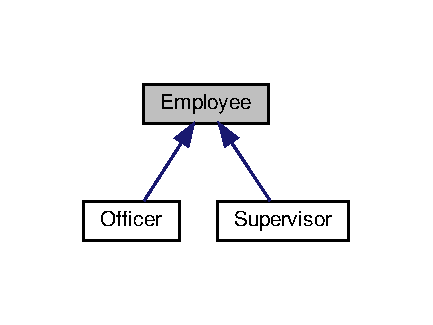
\includegraphics[width=208pt]{classEmployee__inherit__graph}
\end{center}
\end{figure}
\subsection*{Public Member Functions}
\begin{DoxyCompactItemize}
\item 
virtual void \hyperlink{classEmployee_a79556ad700627dba88049f487a34a762}{print} ()
\item 
virtual double \hyperlink{classEmployee_a01c2c44e15434237db28832f6972e960}{calculate\+Pay} ()
\item 
void \hyperlink{classEmployee_a67c345031cf63f515fb09dc675dee5f3}{anniversary} ()
\item 
\hyperlink{classEmployee_a003c7bd08c40924e381eb0750cbb906f}{Employee} ()
\item 
\hyperlink{classEmployee_ad0c935ef9a290a82dcf7865172c90148}{Employee} (int ID, int years, double hourly\+Rate, float hours\+Worked)
\end{DoxyCompactItemize}
\subsection*{Protected Attributes}
\begin{DoxyCompactItemize}
\item 
\mbox{\Hypertarget{classEmployee_ac31134abb9b4004fc015e51ef579b069}\label{classEmployee_ac31134abb9b4004fc015e51ef579b069}} 
double {\bfseries hourly\+Rate}
\item 
\mbox{\Hypertarget{classEmployee_afde35c73d02eb1cfe89e23a80998b42e}\label{classEmployee_afde35c73d02eb1cfe89e23a80998b42e}} 
float {\bfseries hours\+Worked}
\end{DoxyCompactItemize}
\subsection*{Private Attributes}
\begin{DoxyCompactItemize}
\item 
\mbox{\Hypertarget{classEmployee_a832bbae4ee8a704b917f82c4d497bbac}\label{classEmployee_a832bbae4ee8a704b917f82c4d497bbac}} 
int {\bfseries ID}
\item 
\mbox{\Hypertarget{classEmployee_a3e4862d9dfc73becb459a562fa2e25f5}\label{classEmployee_a3e4862d9dfc73becb459a562fa2e25f5}} 
int {\bfseries years}
\end{DoxyCompactItemize}


\subsection{Detailed Description}
Stores and calculates basic employee information. 

\hyperlink{classEmployee}{Employee} main class, holds basic employee information 

\subsection{Constructor \& Destructor Documentation}
\mbox{\Hypertarget{classEmployee_a003c7bd08c40924e381eb0750cbb906f}\label{classEmployee_a003c7bd08c40924e381eb0750cbb906f}} 
\index{Employee@{Employee}!Employee@{Employee}}
\index{Employee@{Employee}!Employee@{Employee}}
\subsubsection{\texorpdfstring{Employee()}{Employee()}\hspace{0.1cm}{\footnotesize\ttfamily [1/2]}}
{\footnotesize\ttfamily Employee\+::\+Employee (\begin{DoxyParamCaption}{ }\end{DoxyParamCaption})}

\hyperlink{classEmployee}{Employee} class default constructor.

\begin{DoxyPrecond}{Precondition}
An \hyperlink{classEmployee}{Employee} 
\end{DoxyPrecond}
\begin{DoxyPostcond}{Postcondition}
An empty \hyperlink{classEmployee}{Employee} will be generated, hollow like the rest of us. 
\end{DoxyPostcond}
\mbox{\Hypertarget{classEmployee_ad0c935ef9a290a82dcf7865172c90148}\label{classEmployee_ad0c935ef9a290a82dcf7865172c90148}} 
\index{Employee@{Employee}!Employee@{Employee}}
\index{Employee@{Employee}!Employee@{Employee}}
\subsubsection{\texorpdfstring{Employee()}{Employee()}\hspace{0.1cm}{\footnotesize\ttfamily [2/2]}}
{\footnotesize\ttfamily Employee\+::\+Employee (\begin{DoxyParamCaption}\item[{int}]{ID,  }\item[{int}]{years,  }\item[{double}]{hourly\+Rate,  }\item[{float}]{hours\+Worked }\end{DoxyParamCaption})}

\hyperlink{classEmployee}{Employee} class paramaterized constructor.


\begin{DoxyParams}{Parameters}
{\em int} & ID \hyperlink{classEmployee}{Employee} ID \\
\hline
{\em int} & years Years \hyperlink{classEmployee}{Employee} has worked \\
\hline
{\em double} & hourly\+Rate \hyperlink{classEmployee}{Employee} Hourly Pay \\
\hline
{\em float} & hours\+Worked \hyperlink{classEmployee}{Employee} Hours Working \\
\hline
\end{DoxyParams}
\begin{DoxyPrecond}{Precondition}
An \hyperlink{classEmployee}{Employee} 
\end{DoxyPrecond}
\begin{DoxyPostcond}{Postcondition}
An \hyperlink{classEmployee}{Employee} with the given information will be generated. 
\end{DoxyPostcond}


\subsection{Member Function Documentation}
\mbox{\Hypertarget{classEmployee_a67c345031cf63f515fb09dc675dee5f3}\label{classEmployee_a67c345031cf63f515fb09dc675dee5f3}} 
\index{Employee@{Employee}!anniversary@{anniversary}}
\index{anniversary@{anniversary}!Employee@{Employee}}
\subsubsection{\texorpdfstring{anniversary()}{anniversary()}}
{\footnotesize\ttfamily void Employee\+::anniversary (\begin{DoxyParamCaption}{ }\end{DoxyParamCaption})}

A method that increments an \hyperlink{classEmployee}{Employee}\textquotesingle{}s years by 1 and increases their hourly\+Rate by 2\%. Also prints a congratulatory statement.

\begin{DoxyPrecond}{Precondition}
A good \hyperlink{classEmployee}{Employee} 
\end{DoxyPrecond}
\begin{DoxyReturn}{Returns}
void 
\end{DoxyReturn}
\begin{DoxyPostcond}{Postcondition}
The given \hyperlink{classEmployee}{Employee} will be given a 2\% hourly\+Rate increase for their continued year of work. 
\end{DoxyPostcond}


Referenced by run\+Employee\+Tests().

\mbox{\Hypertarget{classEmployee_a01c2c44e15434237db28832f6972e960}\label{classEmployee_a01c2c44e15434237db28832f6972e960}} 
\index{Employee@{Employee}!calculate\+Pay@{calculate\+Pay}}
\index{calculate\+Pay@{calculate\+Pay}!Employee@{Employee}}
\subsubsection{\texorpdfstring{calculate\+Pay()}{calculatePay()}}
{\footnotesize\ttfamily double Employee\+::calculate\+Pay (\begin{DoxyParamCaption}{ }\end{DoxyParamCaption})\hspace{0.3cm}{\ttfamily [virtual]}}

A method that calculates pay by multiplying hourly\+Rate $\ast$ hours\+Worked.

\begin{DoxyPrecond}{Precondition}
An \hyperlink{classEmployee}{Employee} 
\end{DoxyPrecond}
\begin{DoxyReturn}{Returns}
virtual double The \hyperlink{classEmployee}{Employee}\textquotesingle{}s pay. 
\end{DoxyReturn}
\begin{DoxyPostcond}{Postcondition}

\end{DoxyPostcond}


Reimplemented in \hyperlink{classOfficer_a1fa1aad39b9e95be7a088990ebf17059}{Officer}, and \hyperlink{classSupervisor_aa37daa89523c08b84ae8141299e036f8}{Supervisor}.



Referenced by Supervisor\+::calculate\+Pay(), and run\+Employee\+Tests().

\mbox{\Hypertarget{classEmployee_a79556ad700627dba88049f487a34a762}\label{classEmployee_a79556ad700627dba88049f487a34a762}} 
\index{Employee@{Employee}!print@{print}}
\index{print@{print}!Employee@{Employee}}
\subsubsection{\texorpdfstring{print()}{print()}}
{\footnotesize\ttfamily void Employee\+::print (\begin{DoxyParamCaption}{ }\end{DoxyParamCaption})\hspace{0.3cm}{\ttfamily [virtual]}}

Prints all basic employee information.

\begin{DoxyPrecond}{Precondition}
An \hyperlink{classEmployee}{Employee} 
\end{DoxyPrecond}
\begin{DoxyReturn}{Returns}
virtual 
\end{DoxyReturn}
\begin{DoxyPostcond}{Postcondition}
prints all employee info to console. 
\end{DoxyPostcond}


Reimplemented in \hyperlink{classOfficer_aeadece05a1a0b7fb29bd412830d2e07a}{Officer}, and \hyperlink{classSupervisor_a92483dc9a54904d79b46c6ec4efb3f54}{Supervisor}.



Referenced by Officer\+::print(), Supervisor\+::print(), and run\+Employee\+Tests().



The documentation for this class was generated from the following files\+:\begin{DoxyCompactItemize}
\item 
\hyperlink{Employee_8h}{Employee.\+h}\item 
\hyperlink{Employee_8cpp}{Employee.\+cpp}\end{DoxyCompactItemize}

\hypertarget{classOfficer}{}\section{Officer Class Reference}
\label{classOfficer}\index{Officer@{Officer}}


Stores and calculates \hyperlink{classOfficer}{Officer} information.  




{\ttfamily \#include \char`\"{}Doxygen-\/\+Test/\+Officer.\+h\char`\"{}}



Inheritance diagram for Officer\+:
\nopagebreak
\begin{figure}[H]
\begin{center}
\leavevmode
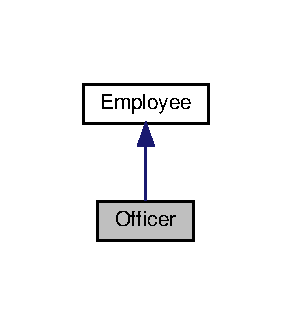
\includegraphics[width=140pt]{classOfficer__inherit__graph}
\end{center}
\end{figure}


Collaboration diagram for Officer\+:
\nopagebreak
\begin{figure}[H]
\begin{center}
\leavevmode
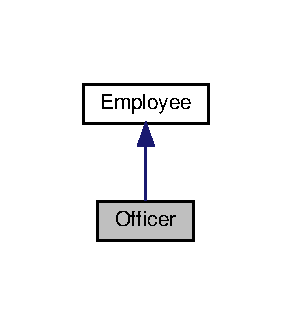
\includegraphics[width=140pt]{classOfficer__coll__graph}
\end{center}
\end{figure}
\subsection*{Public Member Functions}
\begin{DoxyCompactItemize}
\item 
void \hyperlink{classOfficer_aeadece05a1a0b7fb29bd412830d2e07a}{print} ()
\item 
double \hyperlink{classOfficer_a1fa1aad39b9e95be7a088990ebf17059}{calculate\+Pay} ()
\item 
\hyperlink{classOfficer_a80ac1e36a3f36c3a7e12b5dc9320ad89}{Officer} ()
\item 
\hyperlink{classOfficer_ac75c45d6e8628606278cb4ce6596f67f}{Officer} (int ID, int years, double hourly\+Rate, float hours\+Worked, double evilness)
\end{DoxyCompactItemize}
\subsection*{Private Attributes}
\begin{DoxyCompactItemize}
\item 
\mbox{\Hypertarget{classOfficer_a63465c5f16e8148e5bc0a3bb4ecd1781}\label{classOfficer_a63465c5f16e8148e5bc0a3bb4ecd1781}} 
double {\bfseries evilness}
\end{DoxyCompactItemize}
\subsection*{Additional Inherited Members}


\subsection{Detailed Description}
Stores and calculates \hyperlink{classOfficer}{Officer} information. 

Derived \hyperlink{classEmployee}{Employee} class for \hyperlink{classOfficer}{Officer} employees. 

\subsection{Constructor \& Destructor Documentation}
\mbox{\Hypertarget{classOfficer_a80ac1e36a3f36c3a7e12b5dc9320ad89}\label{classOfficer_a80ac1e36a3f36c3a7e12b5dc9320ad89}} 
\index{Officer@{Officer}!Officer@{Officer}}
\index{Officer@{Officer}!Officer@{Officer}}
\subsubsection{\texorpdfstring{Officer()}{Officer()}\hspace{0.1cm}{\footnotesize\ttfamily [1/2]}}
{\footnotesize\ttfamily Officer\+::\+Officer (\begin{DoxyParamCaption}{ }\end{DoxyParamCaption})}

\hyperlink{classOfficer}{Officer} class default constructor.

\begin{DoxyPrecond}{Precondition}
An \hyperlink{classOfficer}{Officer} 
\end{DoxyPrecond}
\begin{DoxyPostcond}{Postcondition}
Creates an empty \hyperlink{classOfficer}{Officer}, not that different from a complete one. 
\end{DoxyPostcond}
\mbox{\Hypertarget{classOfficer_ac75c45d6e8628606278cb4ce6596f67f}\label{classOfficer_ac75c45d6e8628606278cb4ce6596f67f}} 
\index{Officer@{Officer}!Officer@{Officer}}
\index{Officer@{Officer}!Officer@{Officer}}
\subsubsection{\texorpdfstring{Officer()}{Officer()}\hspace{0.1cm}{\footnotesize\ttfamily [2/2]}}
{\footnotesize\ttfamily Officer\+::\+Officer (\begin{DoxyParamCaption}\item[{int}]{ID,  }\item[{int}]{years,  }\item[{double}]{hourly\+Rate,  }\item[{float}]{hours\+Worked,  }\item[{double}]{evilness }\end{DoxyParamCaption})}

\hyperlink{classOfficer}{Officer} class paramaterized constructor.


\begin{DoxyParams}{Parameters}
{\em int} & ID \hyperlink{classOfficer}{Officer} ID \\
\hline
{\em int} & years \hyperlink{classOfficer}{Officer}\textquotesingle{}s Years Worked \\
\hline
{\em double} & hourly\+Rate \hyperlink{classOfficer}{Officer}\textquotesingle{}s Hourly Pay \\
\hline
{\em float} & hours\+Worked \hyperlink{classOfficer}{Officer}\textquotesingle{}s Hours Working \\
\hline
{\em double} & evilness \hyperlink{classOfficer}{Officer}\textquotesingle{}s Evilness \\
\hline
\end{DoxyParams}
\begin{DoxyPrecond}{Precondition}
An \hyperlink{classOfficer}{Officer} 
\end{DoxyPrecond}
\begin{DoxyPostcond}{Postcondition}
An \hyperlink{classOfficer}{Officer} with the given information will be created. 
\end{DoxyPostcond}


\subsection{Member Function Documentation}
\mbox{\Hypertarget{classOfficer_a1fa1aad39b9e95be7a088990ebf17059}\label{classOfficer_a1fa1aad39b9e95be7a088990ebf17059}} 
\index{Officer@{Officer}!calculate\+Pay@{calculate\+Pay}}
\index{calculate\+Pay@{calculate\+Pay}!Officer@{Officer}}
\subsubsection{\texorpdfstring{calculate\+Pay()}{calculatePay()}}
{\footnotesize\ttfamily double Officer\+::calculate\+Pay (\begin{DoxyParamCaption}{ }\end{DoxyParamCaption})\hspace{0.3cm}{\ttfamily [virtual]}}

Calculates \hyperlink{classOfficer}{Officer} pay\+: (hourly\+Rate $\ast$ hours\+Worked + evilness)

\begin{DoxyPrecond}{Precondition}
An \hyperlink{classOfficer}{Officer} 
\end{DoxyPrecond}
\begin{DoxyReturn}{Returns}
double The \hyperlink{classOfficer}{Officer}\textquotesingle{}s pay. 
\end{DoxyReturn}
\begin{DoxyPostcond}{Postcondition}

\end{DoxyPostcond}


Reimplemented from \hyperlink{classEmployee_a01c2c44e15434237db28832f6972e960}{Employee}.

\mbox{\Hypertarget{classOfficer_aeadece05a1a0b7fb29bd412830d2e07a}\label{classOfficer_aeadece05a1a0b7fb29bd412830d2e07a}} 
\index{Officer@{Officer}!print@{print}}
\index{print@{print}!Officer@{Officer}}
\subsubsection{\texorpdfstring{print()}{print()}}
{\footnotesize\ttfamily void Officer\+::print (\begin{DoxyParamCaption}{ }\end{DoxyParamCaption})\hspace{0.3cm}{\ttfamily [virtual]}}

Prints all basic employee information alongside Officer-\/specific information.

\begin{DoxyPrecond}{Precondition}
An \hyperlink{classOfficer}{Officer} 
\end{DoxyPrecond}
\begin{DoxyReturn}{Returns}
void 
\end{DoxyReturn}
\begin{DoxyPostcond}{Postcondition}
Prints all \hyperlink{classOfficer}{Officer} information 
\end{DoxyPostcond}


Reimplemented from \hyperlink{classEmployee_a79556ad700627dba88049f487a34a762}{Employee}.



The documentation for this class was generated from the following files\+:\begin{DoxyCompactItemize}
\item 
\hyperlink{Officer_8h}{Officer.\+h}\item 
\hyperlink{Officer_8cpp}{Officer.\+cpp}\end{DoxyCompactItemize}

\hypertarget{classSupervisor}{}\section{Supervisor Class Reference}
\label{classSupervisor}\index{Supervisor@{Supervisor}}


Inheritance diagram for Supervisor\+:\nopagebreak
\begin{figure}[H]
\begin{center}
\leavevmode
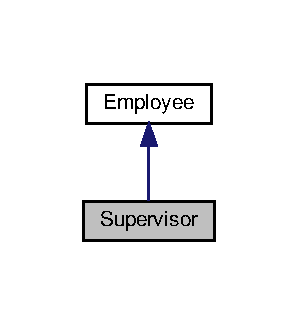
\includegraphics[width=143pt]{classSupervisor__inherit__graph}
\end{center}
\end{figure}


Collaboration diagram for Supervisor\+:\nopagebreak
\begin{figure}[H]
\begin{center}
\leavevmode
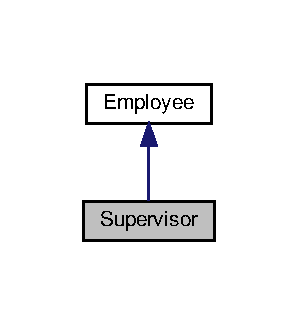
\includegraphics[width=143pt]{classSupervisor__coll__graph}
\end{center}
\end{figure}
\subsection*{Public Member Functions}
\begin{DoxyCompactItemize}
\item 
\mbox{\Hypertarget{classSupervisor_a92483dc9a54904d79b46c6ec4efb3f54}\label{classSupervisor_a92483dc9a54904d79b46c6ec4efb3f54}} 
void {\bfseries print} ()
\item 
\mbox{\Hypertarget{classSupervisor_aa37daa89523c08b84ae8141299e036f8}\label{classSupervisor_aa37daa89523c08b84ae8141299e036f8}} 
double {\bfseries calculate\+Pay} ()
\item 
\mbox{\Hypertarget{classSupervisor_a02d9245744652deb20e9408001d6ed3b}\label{classSupervisor_a02d9245744652deb20e9408001d6ed3b}} 
{\bfseries Supervisor} (int ID, int years, double hourly\+Rate, float hours\+Worked, int num\+Supervised)
\end{DoxyCompactItemize}
\subsection*{Private Attributes}
\begin{DoxyCompactItemize}
\item 
\mbox{\Hypertarget{classSupervisor_af8b7097d8147c93a68d1f63c5b898797}\label{classSupervisor_af8b7097d8147c93a68d1f63c5b898797}} 
int {\bfseries num\+Supervised}
\end{DoxyCompactItemize}
\subsection*{Additional Inherited Members}


The documentation for this class was generated from the following files\+:\begin{DoxyCompactItemize}
\item 
Supervisor.\+h\item 
Supervisor.\+cpp\end{DoxyCompactItemize}

%--- End generated contents ---

% Index
\backmatter
\newpage
\phantomsection
\clearemptydoublepage
\addcontentsline{toc}{chapter}{Index}
\printindex

\end{document}
